\begin{savequote}[8cm]
It's simple mathematics.
  \qauthor{--- Mos Def, \textit{Mathematics}}
\end{savequote}

\chapter{\label{ch:2-litreview}Simulation of hybrid halide perovskites}

The text and figures in this chapter are adapted from \href{https://doi.org/10.1063/1.4984964}{Whalley, L. D., Frost, J. M., Jung, Y. -K. and Walsh, A. (2017). Perspective: Theory and simulation of hybrid halide perovskites. \textit{The Journal of Chemical Physics}, 146(22), p.220901.} © 2017 CC-BY

\section{Introduction}

In this chapter I address recent progress and current challenges in the theory and simulation of hybrid perovskites. 
Particular attention is paid to predicting properties that assess the photovoltaic potential of a material. 
Factors to consider include: light absorption, charge transport, absolute band energies, defect physics and chemical stability. 

The perovskite mineral, \ce{CaTiO3}, is the archetype for the structure of many functional materials.\autocite{Schaak2002}
Metal halide perovskites have been studied for their semiconducting properties since the 1950s\autocite{Moller1958}; 
yet only recently have organic-inorganic perovskites such as \ce{CH3NH3PbI3} (MAPI) been applied to solar energy conversion, showing remarkably strong photovoltaic action for a solution processed material.\autocite{Kojima2009}
The field has progressed rapidly in the past eight years, with the increase in power conversion efficiency supported by over three thousand research publications.\autocite{Stranks2015b,Saparov2016b,Park2016,Walsh2016,Wallace2017}
Other potential application areas of these materials include 
thermoelectrics,\autocite{He2014,Mettan2015}
light-emitting diodes,\autocite{Protesescu2015,Stranks2015b}
and
solid-state memory.\autocite{Yoo2015a,Liu2017}

These materials combine a complex crystal structure, modulated by static and dynamic disorder, with an electronic structure requiring methods beyond density functional theory to treat many-body and relativistic effects. 
As such, the halide perovskites represent a challenge to predictive materials modelling. 
% https://www.youtube.com/watch?v=fAnP2ck-7o4

\begin{figure*}
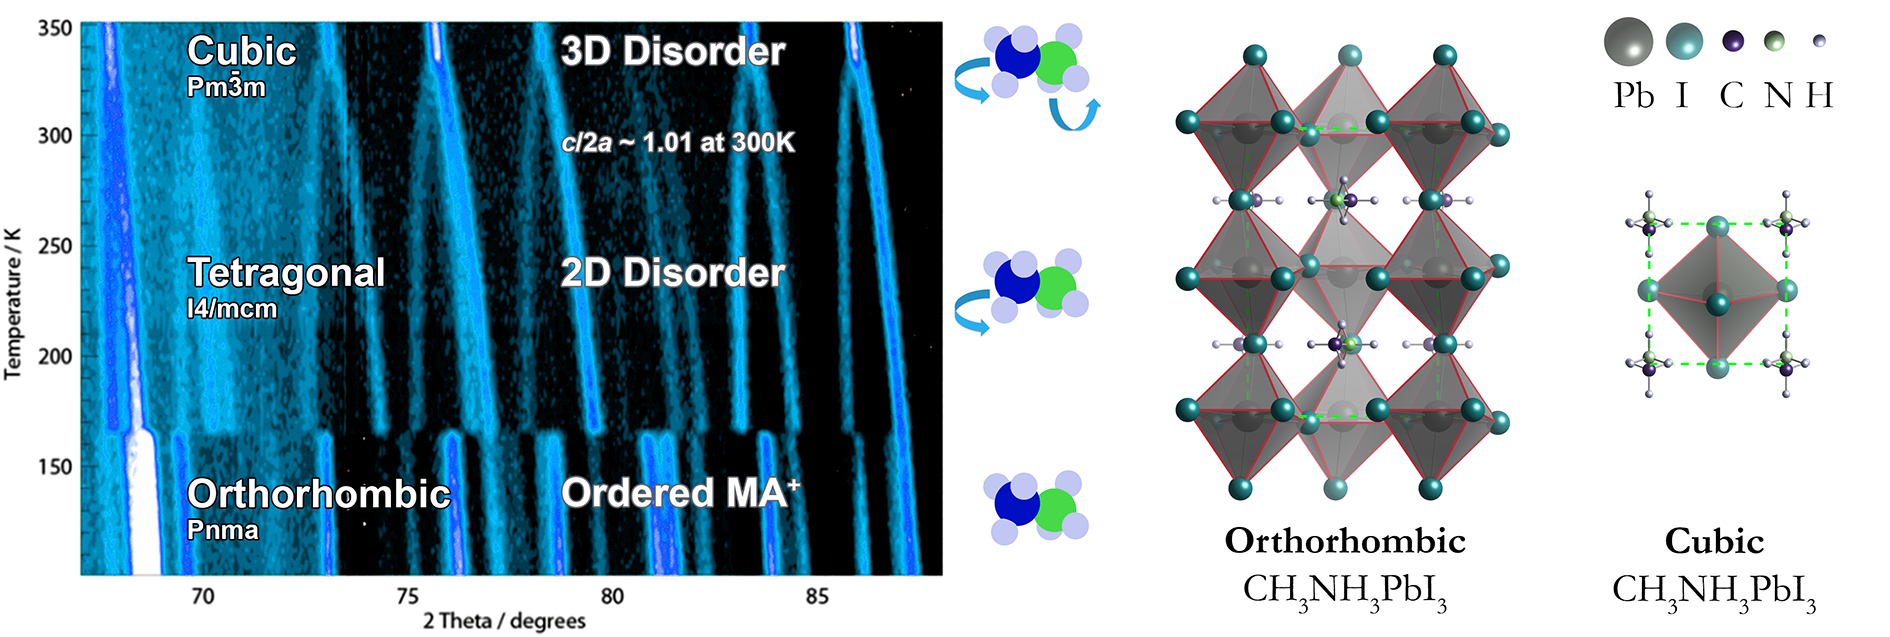
\includegraphics[width=1.0\columnwidth]{./figures/ch2/f1.png}
\caption[\ce{CH3NH3PbI3} powder neutron diffraction pattern and crystallographic unit cells]{
The high-resolution powder neutron diffraction pattern of the hybrid halide perovskite \ce{CH3NH3PbI3} is shown in the left panel (adapted with permission from Ref. \autocite{Frost2016a} based on data in Ref. \autocite{Weller2015}), which illustrates the low and high temperature phase transitions. While an ordered \ce{CH3NH3+} sub-lattice is expected in the orthorhombic phase, orientation disorder increases with temperature. 
The crystallographic unit cells of the pseudo-cubic and orthorhombic perovskite phases are shown in the right panel (adapted with permission from Ref. \autocite{Brivio2015a}). The associated structure files can be accessed from \url{https://github.com/WMD-group/hybrid-perovskites}. Figure prepared by Aron Walsh.
}
\label{fig1}
\end{figure*}

\section{Crystal structures and lattice dynamics} 

\subsection{Phase diversity}
Hybrid perovskites of the type \ce{ABX3} form a crystal structure with an organic A site cation contained in an inorganic \ce{BX3} framework of corner sharing octahedra. 
Halide substitution on the X site (X = \ce{Cl-}, \ce{Br-}, \ce{I-}), metal substitutions on the B site (B = \ce{Pb^2+}, \ce{Sn^2+}), and cation substitution on the A site (A = \ce{CH3NH3+}, \ce{HC(NH2)2+}, \ce{Cs+}, \ce{Rb+}) lead to various chemical and physical properties.\autocite{Mitzi2001,Mitzi2004a}
In addition to isoelectronic substitutions (e.g. replacing \ce{Pb^2+} by \ce{Sn^2+}), it is possible to perform pairwise substitutions to form double perovskites (e.g. replacing \ce{2Pb^2+} by \ce{Bi^3+} and \ce{Ag^+}).\autocite{Savory2016,Volonakis2016}

In the first report of MAPI by Weber in 1978, the crystal structure was assigned as cubic perovskite (space group $Pm\bar{3}m$).\autocite{Weber1978,Weber1978a}
The anionic \ce{PbI3-} network is charge balanced by the  \ce{CH3NH3+} molecular cation.
The symmetry of \ce{CH3NH3+}  ($C_{3v}$) is incompatible with the space group symmetry ($O_h$) unless orientation disorder (static or dynamic) is present.
The crystal structure solved from X-ray or neutron diffraction data usually spread the molecules over a number of orientations with partial occupancy of the associated lattice sites.
A common feature of perovskites is the existence of phase changes during heating (typically from lower to higher symmetry) as shown in Figure \ref{fig1}. 
In hybrid halides containing methylammonium, these are orthorhombic ($Pnma$), tetragonal ($I4/mcm$) and cubic ($Pm\bar{3}m$) phases.\autocite{Weller2015} 
%
For MAPI the $Pnma$ to $I4/mcm$ phase transition is first-order with an associated discontinuity in physical properties, while the $I4/mcm$ to $Pm\bar{3}m$ phase transition is second-order with a continuous evolution of the structure and properties.\autocite{Onoda-Yamamuro1990,Weller2015}

The phase transitions are linked to a change in the tilting pattern of the inorganic octahedral cages, and order-disorder transitions of the molecular sub-lattice.\autocite{Onoda-Yamamuro1990,Yamamuro1992a,Onoda-yamamuro1992}
X-ray diffraction (XRD) measurements upon cooling (heating) suggest the incursion of tetragonal in orthorhombic phases (and vice versa),\autocite{Hutter2016a}
which is common for first-order solid-state phase transitions. 

Similar phase behaviour tends to be seen for other compositions; however, the transition temperatures vary.
In MAPI the orthorhombic to tetragonal transition temperature is $162$ K, becoming cubic by around $328$ K,
while \ce{CH3NH3PbBr3} is cubic above $237$ K.\autocite{Poglitsch1987c} 
%

\begin{figure*}
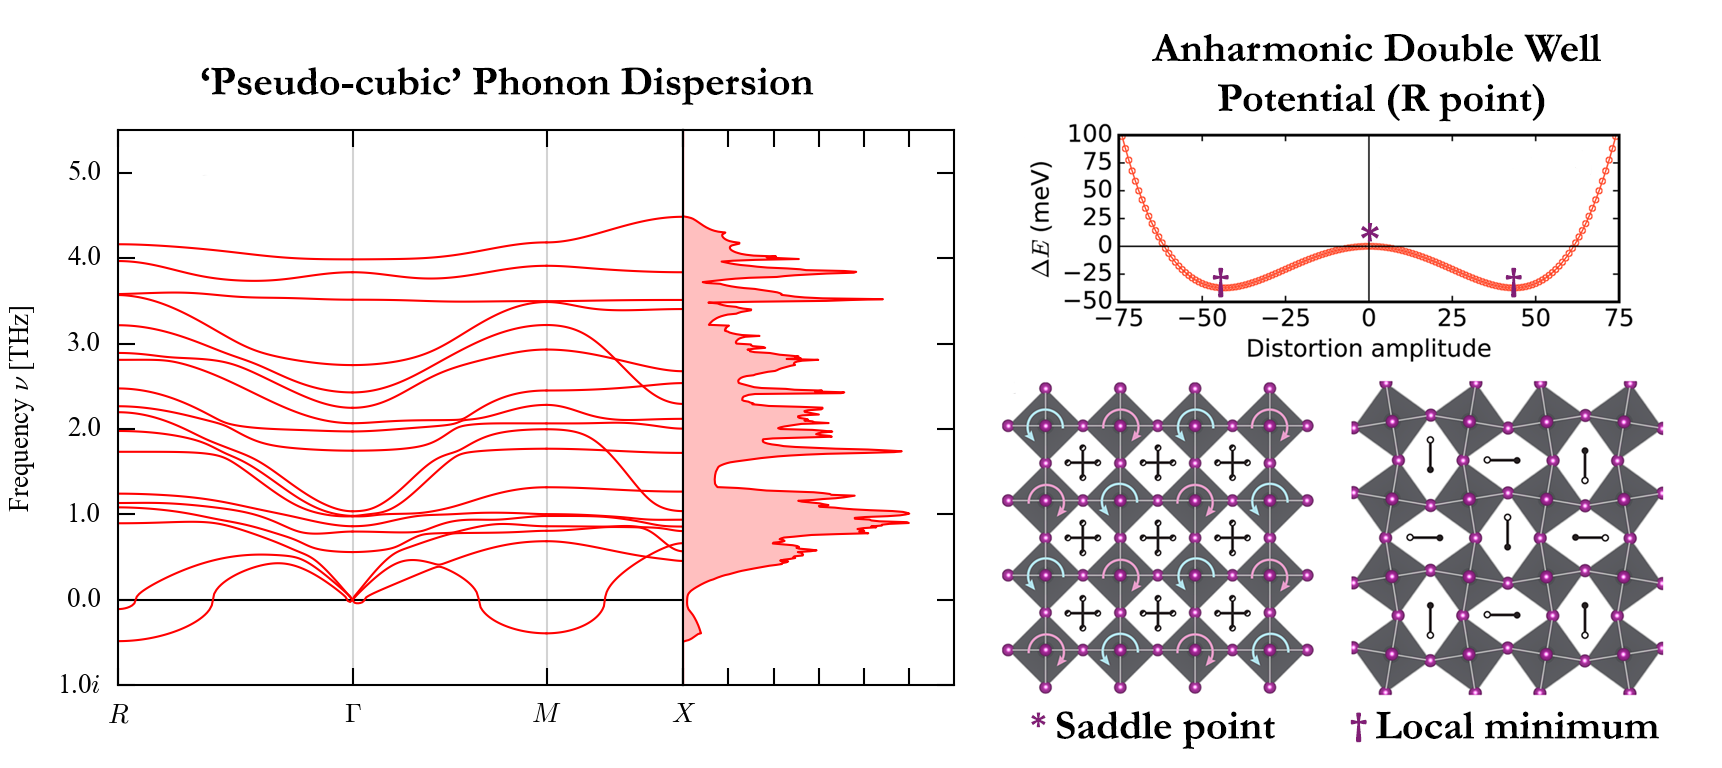
\includegraphics[width=1.0\columnwidth]{./figures/ch2/f2.png}
\caption[\ce{CH3NH3PbI3} phonon dispersion and double-well potential energy surface]{
    (Left) The harmonic phonon dispersion for \ce{CH3NH3PbI3} from a `pseudo-cubic' structure. 
    The imaginary frequencies of acoustic modes at the $M$ ($q=\frac{1}{2},\frac{1}{2},0$) and $R$ ($q = \frac{1}{2}, \frac{1}{2}, \frac{1}{2}$) Brillouin zone boundary correspond to an instability expressible in a supercell as alternate tilting of the octahedra.
    (Right) Following the imaginary acoustic mode at the $R$ Brillouin zone boundary in a $2\times2\times2$ supercell expansion shows a double-well potential in the DFT internal energy. 
    The saddle point corresponds to a $1\times1\times1$ cubic structure, whilst the two local minima correspond to a distorted structure of lower symmetry. 
The energy barrier is small enough to allow both minima can be accessed at room temperature, so the system is expected to exhibit dynamic rather than static disorder. 
Similar behaviour is found at the $M$ point. 
Figure adapted by Aron Walsh with permission from Refs. \cite{Whalley2016} and \cite{Beecher2016a}.
The underlying phonon data is available from \url{https://github.com/WMD-group/Phonons}.
}
\label{fig2}
\end{figure*}

\subsection{Local and average crystal environment} \label{localaverage}

The first electronic structure calculation of hybrid halide perovskites was by Chang, Park and Matsuishi in 2004, \autocite{Chang2004}
in the local density approximation (LDA) of density functional theory (DFT).
They modelled a static structure where the \ce{CH3NH3+} molecule was aligned along $\langle100\rangle$ (towards the face of the corner-sharing \ce{PbI3-} framework), but found that the barrier for rotation to $\langle111\rangle$ was less than $10$ meV. 
This small barrier for cation rotation gave credence to a prior model that the molecular sub-lattice was dynamically disordered.\autocite{Poglitsch1987c}
Similar barriers were later found within the generalised gradient approximation (GGA) of DFT.\autocite{Brivio2013} 
%JMF: Bit of a 'me too' citation? Anything extra to add? - AW: Unfortunately not, and we had missed the ealier paper at that time :(

\emph{Ab initio} molecular dynamics (MD), neutron scattering\autocite{Leguy2015b,Chen2015s} and time-resolved infra-red\autocite{Bakulin2015a} data all indicate a 1--10 picosecond reorientation process at room temperature.
As a result of anharmonic molecular rotation, and large-scale dynamic distortions along soft 
vibrational modes, the local structure can deviate considerably from that sampled by diffraction techniques, which do not probe local disorder that preserves long-range order on average.

In spite of the larger cation, FAPI appears to possess a similar timescale of rotation to MAPI\autocite{Weller2015b}. 
A lighter halide (and therefore smaller cage) results in faster rotation, in spite of the greater steric hindrance.\autocite{selig2017organic}
Together, these data suggest that the molecular rotation is a function of the local inorganic cage tilting, where the relatively insignificant mass of the organic cation follows the pocket distortion. 

The spontaneous distortions can also be observed in the vibrational spectra.
The calculated harmonic phonon dispersion for MAPI in the cubic phase is presented in Figure \ref{fig2}.
The acoustic modes soften as they approach the $M$ ($q = \frac{1}{2}, \frac{1}{2}, 0$) and $R$ ($q = \frac{1}{2}, \frac{1}{2}, \frac{1}{2}$) Brillouin zone boundaries. 
This zone boundary instability can only be realised in an even supercell expansion, where it corresponds to anti-phase tilting between successive unit cells.
This behaviour is characteristic of the perovskite structure,\autocite{Yang2017} and can be described by the Glazer tilt notation.\autocite{Glazer1972,Woodward1997} 
%and has been recently identified as common to all inorganic halide perovskites. %cite ruoxi. 

Within the frozen-phonon approximation the potential energy surface can be traced along the soft acoustic $M$ and $R$ modes. 
In both cases this results in a double well with an energy barrier $\sim k_\mathrm{B}T$ at the saddle point;\autocite{Whalley2016}   
at room temperature the structure is dynamically disordered, with continuous tilting.
Indeed, MD simulations show continuous tilting of MAPI and FAPI at room temperature.\autocite{Frost2014,Quarti2015a,Weller2015b}
%
As temperature decreases, the structural instability condenses via the $R$ point (with an energy barrier of 37 meV) into the lower symmetry tetragonal phase. 
This is followed by condensation of the $M$ point (with an energy barrier of 19 meV) to the orthorhombic phase.\autocite{Whalley2016}

In the static picture -- as in the case of an electronic band structure calculated for a single ionic snapshot -- the organic cation plays no direct role in optoelectronic properties of the material as the molecular electronic levels lie below that of the inorganic framework.
Once motion is considered, the electrostatic and steric interaction between the organic molecule and inorganic framework couples tilting and distortion of the octahedra to the organic cation motion.
These tilts and distortions vary the orbital overlap between states, perturbing the band-structure and band-gap.\autocite{Mosconi2014,Quarti2015a,Whalley2016,Saidi2016}
The electronic structure thus becomes sensitive to temperature, which will be discussed further in Section \ref{ch2epcoupling} and Chapter \ref{ch:5-epcoupling}.

\subsection{Thermodynamic and kinetic stability}

\textit{Ab initio} thermodynamics has emerged as a powerful tool in materials modelling, with the ability to assess the stability of new materials and place them on equilibrium phase diagrams even before experimental data is available. \autocite{Reuter2003,Kim2012,Jackson2015a}
The total energy from DFT calculations approximates the internal energy of the system. 
By including lattice vibration (phonon) and thermal expansion contributions, the Gibbs free energy 
and other thermodynamic derivatives can be evaluated.\autocite{Stoffel2010}
In the context of photovoltaic materials, this has been applied to \ce{Cu2ZnSnS4} 
and used to identify the processing window where a single-phase compound can be grown in equilibrium.\autocite{Jackson2014}

An issue with hybrid perovskites and other metal-organic frameworks is that the calculated heat of formation is close to zero.
The decomposition reaction 
\begin{equation}
\ce{CH3NH3PbI3} \rightarrow \ce{CH3NH3I} + \ce{PbI2}
\end{equation}
has been predicted to be exothermic.
%
Subsequent calorimetric experiments have supported the prediction that hybrid lead halide perovskites are metastable.\autocite{Nagabhushana2016}
%
It is likely that these materials are only formed due to entropic (configurational, vibrational and rotational) contributions
to the free energy.

\begin{figure*} \label{f3}
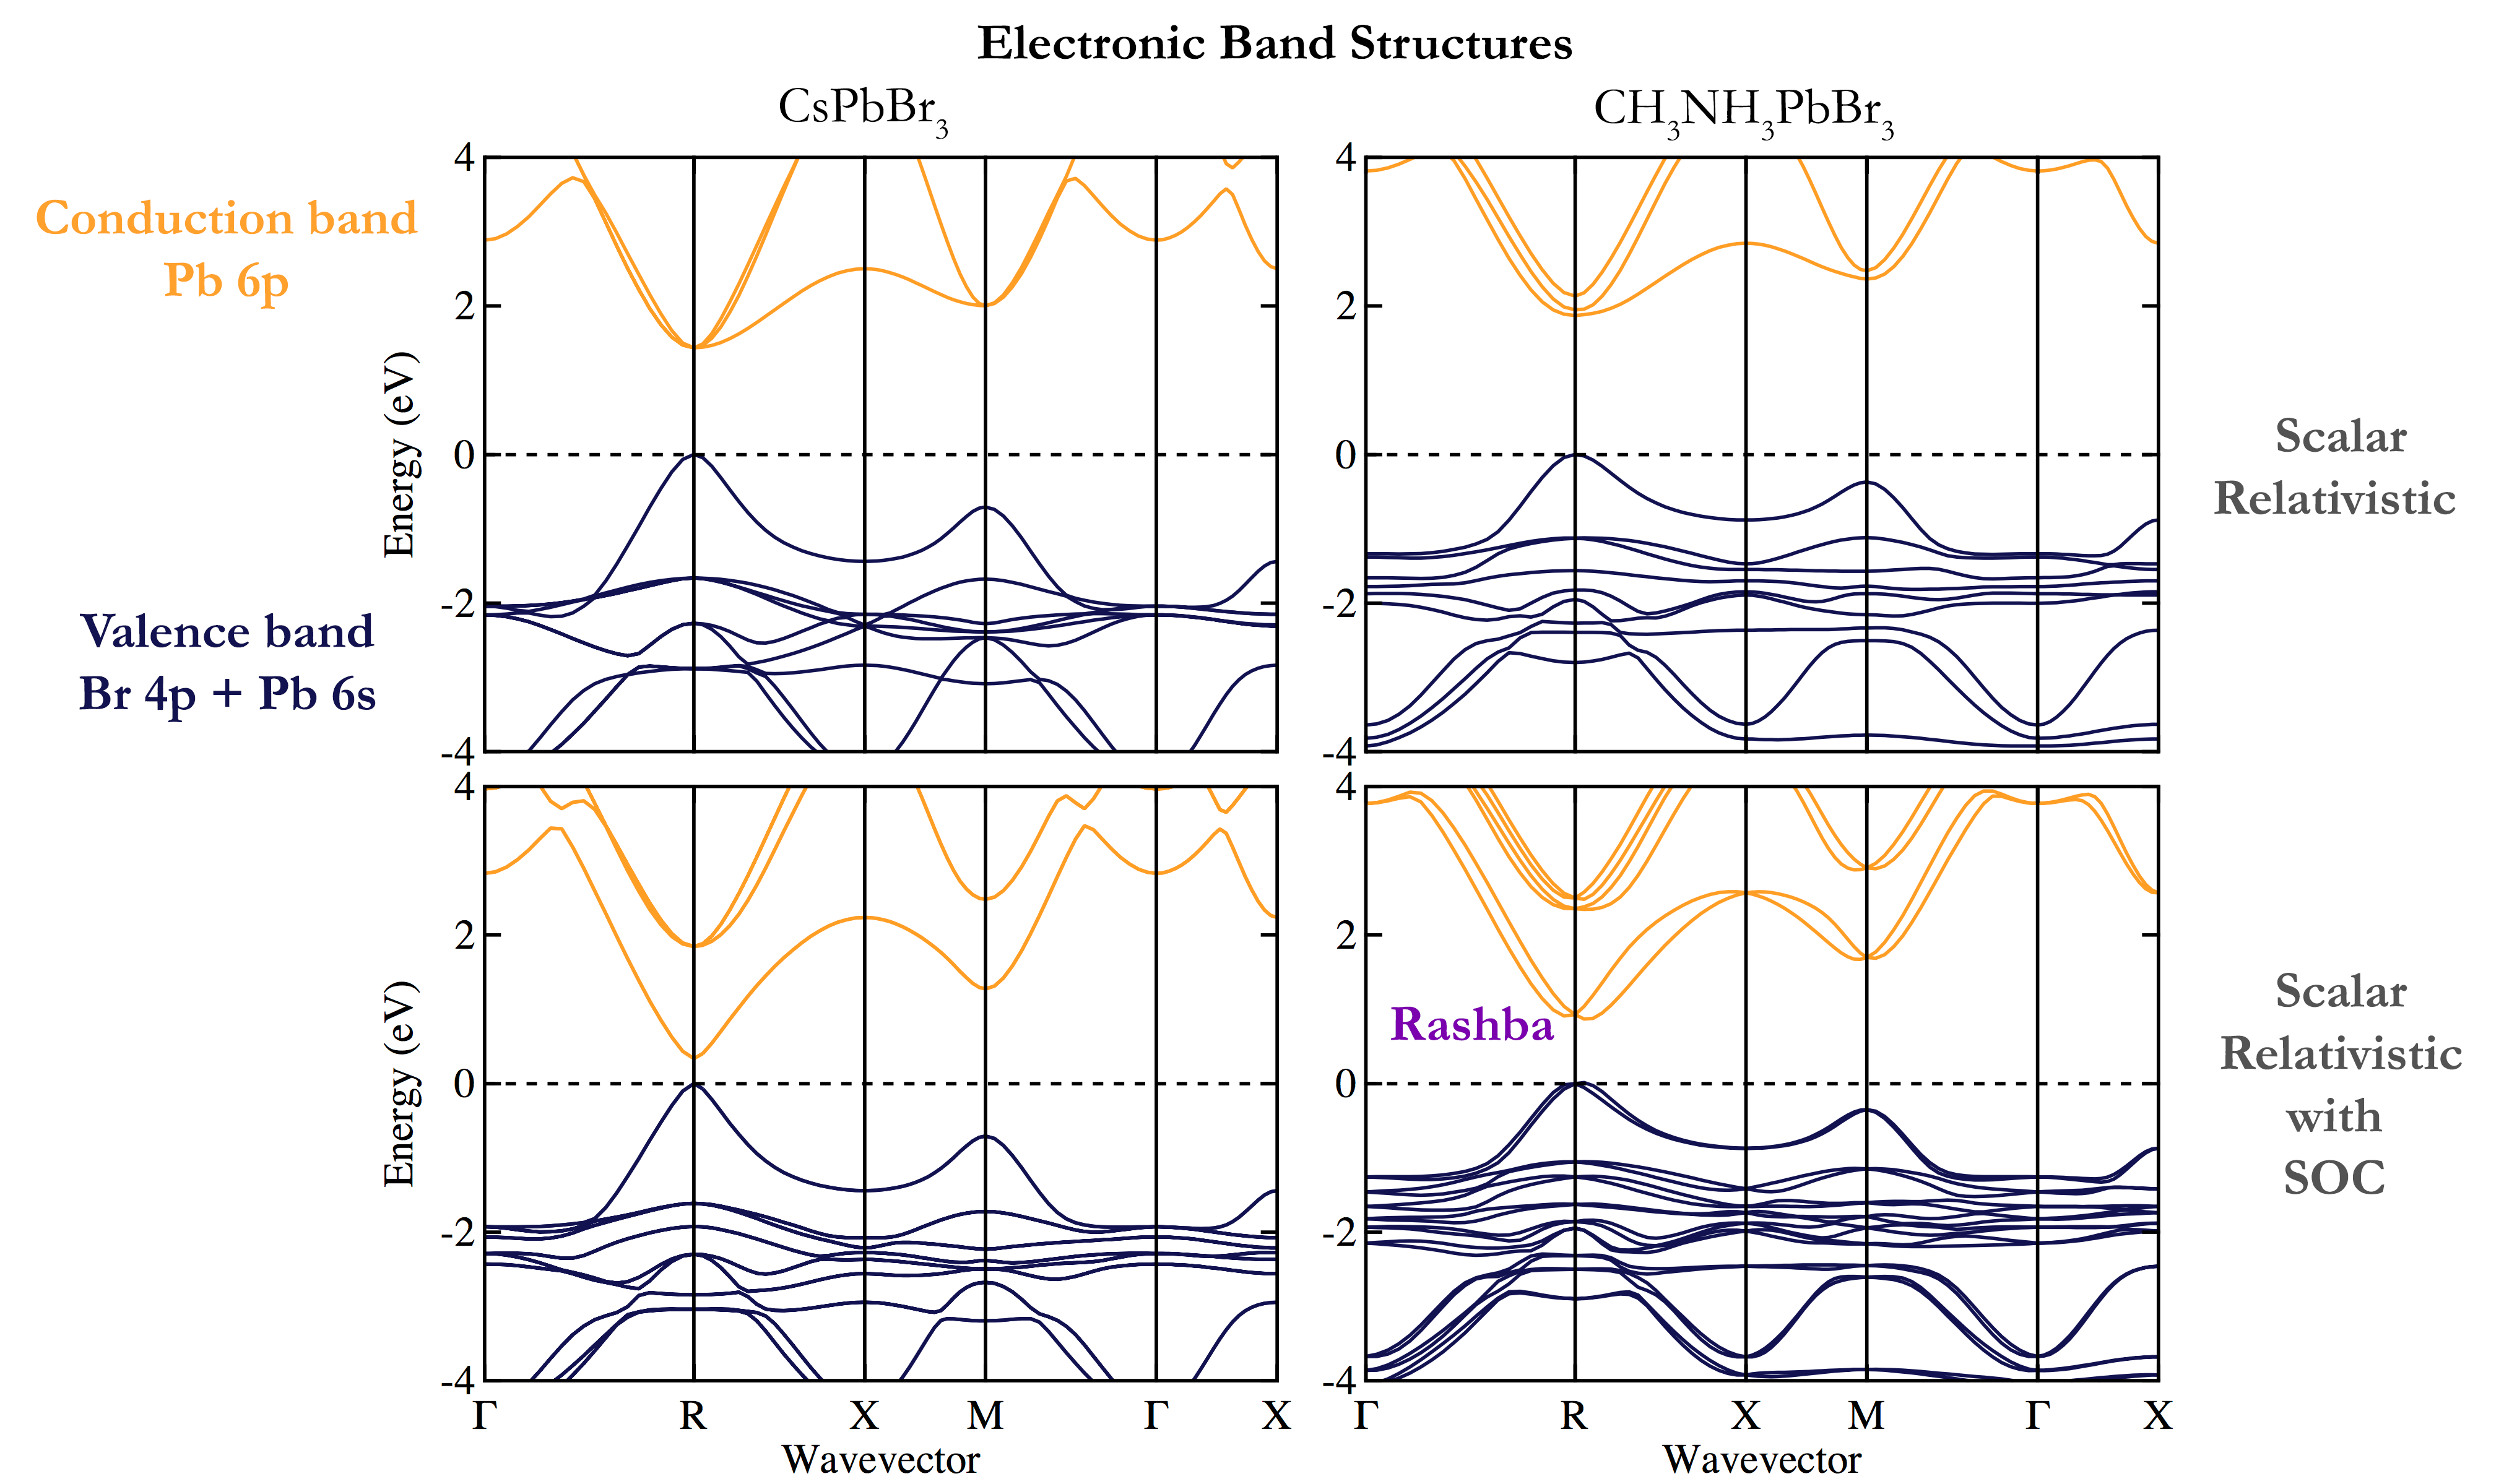
\includegraphics[width=1.0\columnwidth]{./figures/ch2/f3.png}
\caption[Electronic band structures of \ce{CsPbBr3} and \ce{CH3NH3PbBr3}]{
The electronic band structures of the inorganic perovskite \ce{CsPbBr3} and hybrid perovskite \ce{CH3NH3PbBr3} in the cubic phase.
    One effect of the organic cation is to widen the band-gap located at the $R$ point due to the larger lattice constant. 
    Spin-orbit coupling reduces the band-gap in both materials. 
The presence of \ce{CH3NH3+} in the hybrid perovskite results in a non-centrosymmetric crystal, with an associated relativistic Rashba-Dresselhaus splitting of the lower conduction band.
While labels of the special points are those of the cubic perovskite structure (space group $Pm\bar{3}m$),  
    the static model of the hybrid perovskite formally has  \textit{P1} symmetry . 
Points equivalent for a cubic crystal (e.g. $M=\frac{1}{2},\frac{1}{2},0$; $M'=0, \frac{1}{2},\frac{1}{2}$;  $M''=\frac{1}{2},0,\frac{1}{2}$) are inequivalent here. Figure prepared by Young-Kwang Jung.
}
\label{fig3}
\end{figure*}

\subsection{Anharmonic lattice vibrations and thermal conductivity} \label{ch2anharmonic}

Kohn-Sham density functional theory is most often carried out in the Born-Oppenheimer approximation where the nuclei are static classical point charges. 
To consider thermal vibrations, expansion or heat flow the theoretical framework of lattice dynamics can be used.\autocite{Stoffel2010} 
 
In the harmonic approximation, the lattice dynamics are fully specified by second-order force-constants of individual atoms, which are then used to build the dynamical matrix. 
The eigenstates of this matrix are the normal modes of vibration with an associated phonon energy. 
Thermal expansion coefficients, system anharmonicity (e.g. \grun parameters) and the temperature-dependence of other properties can be calculated in the quasi-harmonic approximation (QHA). 
Here the lattice dynamics are harmonic at a given temperature; however, the cell volume is scaled by thermal expansion to give the first-order contribution of finite temperature effects. 

The thermal expansion coefficient of MAPI in the cubic phase has been calculated with the QHA.
The value is sensitive to the density functional used.
For example, a value of $3.0 \times 10^{-5} /K$ is calculated with the PBE functional with Tkatchenko-Scheffler dispersion corrections,\autocite{Saidi2016} while the PBEsol functional produces a value of $12.5 \times 10^{-5} /K$.\autocite{Brivio2015a} 
These compare to finite temperature scattering measures of $1.91 \times 10^{-5} /K$ by X-ray,\autocite{Baikie2013} and $13.2 \times 10^{-5} /K$ by neutron diffraction.\autocite{Weller2015} 
Even taking the smallest value above, the expansion coefficient is one order of magnitude greater than silicon,\autocite{Madelung2004} highlighting the strong deviation from harmonic behaviour in halide perovskites.

In the harmonic approximation (and similarly the QHA), the dynamic matrix eigenmodes are orthogonal and the resulting phonons are non-interacting.
Consequently phonon lifetimes are infinite as the phonons do not scatter; thermal conductivity is infinite. 
To calculate phonon-phonon scattering, and so its contribution to finite thermal conductivity, anharmonic lattice dynamics need to be considered.
A computational route is to use perturbative many-body expansion, e.g. as implemented in \textsc{PHONO3PY},\autocite{Togo2015} which includes third-order force constants. 
For MAPI, 41,544 force evaluations are required for these third-order force constants, compared to 72 for second-order (harmonic) force constants.\autocite{Whalley2016}
Consequently, these calculations are vastly more expensive. 
Using this approach phonon-phonon scattering rates are calculated to be three times larger in MAPI compared to standard covalent semiconductors \ce{CdTe} and \ce{GaAs}.\autocite{Whalley2016} 
Consequently, mean free paths are on the nanometer rather than more typical micrometer scale. 
Lattice thermal conductivity is extremely low, 0.05 Wm$^{-1}$K$^{-1}$ at 300 K.\autocite{Whalley2016}
This combination of high electrical and low thermal conductivity makes these compounds potential thermoelectric materials.\autocite{He2014,Mettan2015}

In highly anharmonic systems third-order force constants and perturbation theory may not be sufficient
to describe the true dynamics, but going further with lattice dynamics becomes prohibitive.
Besides, it is not obvious whether the fundamental tenant of lattice dynamics, of expanding in small displacements around a minimum structure, is correct for these soft and highly anharmonic materials. 
In contrast, MD treats anharmonic contributions to all orders. As MD stochastically explores the phase space, long integration times are required to sample rare events, and finite size effects mean that only phonon modes commensurate with the supercell are sampled.  
%% Low thermal conductivity is linked to material breakdown explains why all of their perovskite LEDs break very quickly (heat builds up and kills the material) - much higher currents than solar cells
% Thermal stability: aron says good article on latest advances: https://pubs.acs.org/doi/10.1021/acs.jpclett.8b00463
\section{Electronic structure}

Despite the dynamic disorder just discussed, in many respects halide perovskites display characteristics of traditional inorganic semiconductors, with a well-defined electronic band structure and electron/hole dispersion relations.
However, when the electronic structure is correctly modelled, various subtleties emerge. 

\subsection{Many-body and relativistic effects} \label{Mbre}

Perhaps surprisingly, local and semi-local exchange-correlation functionals 
provide a reasonable estimate for the band-gaps of these heavy metal halide materials.
This is due to a cancellation of errors. 
For Pb-based perovskites, the conduction band has mainly Pb $6p$ character. 
Due to the large nuclear charge, the electronic kinetic energy requires a relativistic
treatment, and spin-orbit coupling (SoC) becomes significant. 
The first-order effect is a reduction in band-gap by as much as 1 eV\autocite{Brivio2014a}, as the degenerate $6p$ orbitals are split and moved apart. 
This is shown in Figure \ref{fig3} for the bromide compounds.
The typical band-gap underestimation of GGA functionals is offset by the absence of relativistic renormalisation.

SoC is not expected to have a large impact on the structural properties of the Pb-based compounds as the (empty) conduction band is mainly affected, and the force on atoms depends on the electron density (occupied orbitals). 
Accurate force-constants can be calculated without SoC considerations.\autocite{PerezOsorio2015a}
%LW - This just claims it gives same qualtatitve picture, don't think valid to cite on this point.
%AW - Fig 6 shows the potential energy surface as a function of functional

There have been a number of electronic structure calculations considering many-body interactions beyond DFT. 
Quasi-particle self-consistent \textit{GW} theory shows that the band dispersion (and so density of states, optical character and effective mass) is considerably affected by both the \textit{GW} electron correlation and SoC.\autocite{Brivio2014a}
Some materials see only a rigid shift of band structure (retaining DFT dispersion relations)\autocite{VanSchilfgaarde2006,Butler2016} but this is not the case for hybrid perovskites.
The effect of SoC on the band dispersion of MAPI is discussed in Chapter \ref{ch:4-effmass}.

A consequence of SoC when combined with a local electric field is the Rashba-Dresselhaus effect, a splitting of bands in momentum space.\autocite{Kepenekian2015}.
This can be understood as an electromagnetic effect, where the magnetic moment (spin) of the electron interacts with a local electric field, to give rise to a force which displaces it in momentum space. 
Up and down spins are displaced in opposite directions, and this displacement is a function (in both size and direction) of the local electric field, which will depend on the local dynamic order. 
For a static structure, this is demonstrated in Figure \ref{fig3} for \ce{CH3NH3PbBr3}. 
Neglecting SoC, the cubic phase has band extrema at the $R$ point (a direct band-gap).
With SoC the valence and conduction band each split into valleys symmetrical around $R$.
The splitting is much more pronounced in the \ce{Pb} $6p$ conduction band (compared to the \ce{Br} $4p$ valence band), as expected from the $Z^4$ dependence of spin-orbit coupling.
This asymmetry in the band extrema results in direct-gap like absorption and indirect-gap like radiative recombination which is discussed later.
For a comparison between SoC and non-SoC bandstructures across a range of materials see Appendix \ref{app:2-bandstructures}.

The relativistic spin-splitting can only occur in crystals that lack a centre of inversion symmetry, a prerequisite for generating a local electric field. 
The cubic representation of \ce{CsPbBr3} has an inversion centre, so while SoC affects the band-gap through the separation of Pb $6p$ into $p_{\frac{1}{2}}$ and  $p_{\frac{3}{2}}$ combinations,
no splitting of the band extrema away from the high symmetry points is observed (see Figure \ref{fig3}).
This is true only for a static cubic structure and, as discussed earlier, hybrid halides will have continuous local symmetry breaking. 

%It is possible that the Rashba characterisitics of hybrid halide perovskites could be exploited for use in an intermediate band solar cell. The recombination protected pockets could produce a region where an appreciable charge density provides flux to a higher energy conduction band \autocite{frost2016b}.

Point defect calculations will be particularly sensitive to the electronic structure method used.
Neglection of SoC and self-interaction errors can result in an incorrect position of the valence or conduction band edges, thus introducing spurious errors in defect energy levels and predicted defect concentrations.
Du\autocite{Du2015} showed how for the case of an iodine vacancy, a deep (0/+) donor level is predicted for GGA without SoC,
while a resonant donor level is predicted for GGA-SoC and HSE-SoC treatments of electron-exchange and correlation.

\subsection{Electron-phonon coupling} \label{ch2epcoupling}

Going beyond the Born-Oppenheimer approximation, the interaction of the electronic structure with vibrations of the lattice can be considered. 
Electron-phonon coupling can perturb the electronic band energies (changing the band-gap), and couple electronic excitations (the hole and electron quasi-particles) into vibrational excitations (phonon quasi-particles). 
In a semiconductor, charge carrier scattering is often dominated by this electron-phonon interaction, and so the strength of these processes set a limiting value on the mobility. 
Electron-phonon coupling is often calculated in a second-order density functional perturbation theory calculated for a static (rigid ion) structure.
In the normal limit, this term is expected to dominate over the first order contribution from the acoustic deformation potential as vibrations are typically small. 

Saidi et al. sampled all non-soft harmonic phonons at the $\Gamma$ point using a Monte Carlo technique,\autocite{Saidi2016} finding significant differences with the standard perturbation theory results.
%
Electron-phonon interactions can be calculated with MD, but as with phonon-phonon scattering, 
achieving convergence with respect to electronic (\textit{k}-point sampling and basis set) 
and vibrational ($q$-point sampling and supercell size), while maintaining sufficient integration time to capture rare processes, is costly.

Recently a `one shot' method has been developed to calculate band-gap renormalization and phonon-assisted optical absorption, and applied to \ce{Si} and \ce{GaAs}.\autocite{Zacharias2016} 
Nuclei positions are carefully chosen as a representative sample from the thermodynamic ensemble, and the electronic structure is needed for this static structure only---a significant increase in computational efficiency. 
Such techniques may provide a promising method to calculate the electron-phonon coupling of complex materials, but they have not yet been tested for the family of hybrid halide perovskites or other more complicated crystal structures.

\subsection{Charge carrier transport}

Charge carrier transport in hybrid halide perovskites is now considered.
The minority-carrier diffusion length is the average length a photo-excited (or electronically-injected) carrier travels before recombining. 
In a photovoltaic device, the diffusion length must be sufficient to reach the contacts.
The minority-carrier diffusion length is a product of the diffusivity $D$ and lifetime $\tau$ of minority charge carriers, $L_d = \sqrt{D\tau}$.

Minority-carrier diffusion lengths in MAPI are reported to be considerably larger than other solution processed semiconductors.\autocite{Li2015zz}
%
Long lifetimes (large $\tau$) can be partly attributed to the `defect-tolerance' of hybrid perovsites (discussed in Section \ref{defects}), reducing the rate of ionised-impurity scattering and non-radiative recombination.  

The effective masses of electrons and holes in hybrid halide perovskites are small.
Given the effective mass of $< 0.2 m_e$,  the carrier mobility of MAPI ($< 100$ \mob) is modest in comparison to conventional semiconductors such as \ce{Si} or \ce{GaAs} ($> 1000$ \mob).\autocite{Stranks2015b}
Carrier mobility must be limited by strong scattering.

Low temperature mobility in this material reduces as a function of temperature as T$^{-1.5}$, which provides circumstantial evidence for being limited by acoustic phonon scattering.\autocite{Karakus2015,Yi2016a}
However, if only the acoustic phonon scattering (which is elastic due to the population of acoustic modes) is considered, the calculated mobility is orders of magnitude larger than experiment. 
A key realisation is that the soft nature of these semiconductors results in optical phonon modes (see Figure \ref{fig2}) below thermal energy.\autocite{Brivio2015a,PerezOsorio2015a}
Optical phonon scattering is inelastic and dominates once the charge carriers have sufficient energy to generate the phonon modes.\autocite{Leguy2016} 
Through solving the Boltzmann transport equation parameterised by DFT calculations, scattering from longitudinal optical phonons is identified as the process limiting mobility at room temperature.\autocite{Wright2016,Filippetti2016}

Mobility will be further limited by scattering from point and extended lattice defects.\autocite{Ball2016}
Fluctuations in electrostatic potential resulting from dynamic disorder provide a macroscopic structure from which carriers will also scatter.\autocite{Frost2014,Ma2014d}

\begin{figure*} 
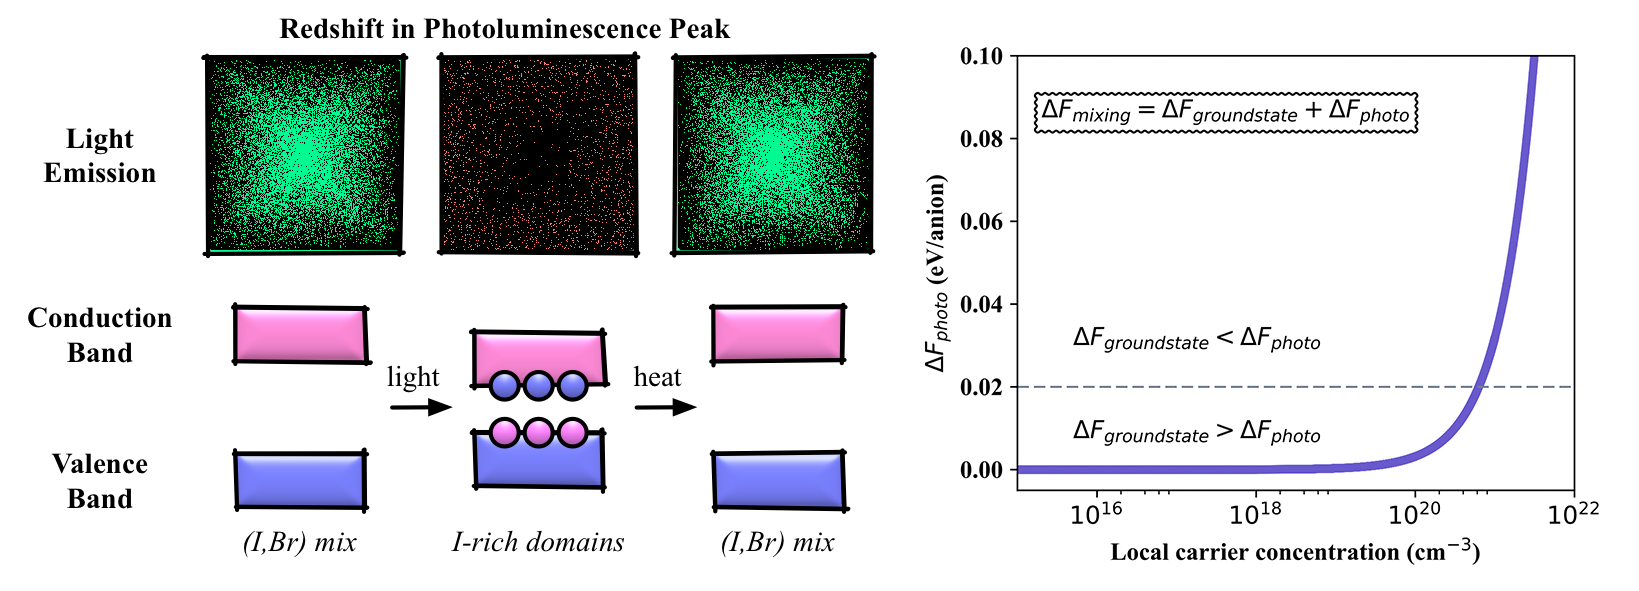
\includegraphics[width=1.0\textwidth]{./figures/ch2/f4.png}
\caption[Simple phase segregation model]{
Halide perovskites are mixed ionic-electronic conductors. The vacancy-mediated diffusion of halide anions has been associated with both current-voltage hysteresis of solar cells and the rapid interchange between iodide, bromide and chloride materials.
One point of controversy remains the reversible ion segregation observed in mixed (Br,I) systems. 
Alloyed materials have been found to phase separate upon illumination, but recover their initial state when the light source is removed. 
The phase separation is associated with a striking red-shift in  photoluminesence spectra.
A statistical mechanical analysis of ground-state DFT calculations suggested a large miscibility gap \autocite{Brivio2016}, while the charge carriers generated upon illumination can provide an additional driving force for phase separation.\autocite{Slotcavage2016}
The results from a simple thermodynamic model are shown in the right panel, where the free energy of mixing contains contributions from the ground-state with an additional component due to the difference in band-gaps between the mixed (I,Br) and phase separated I-rich phases. 
The latter contribution requires local carrier concentrations approaching 10$^{21}$ cm$^{-3}$ to make a substantial contribution to the overall mixing energy. Figure prepared by Aron Walsh.
}
\label{fig4}
\end{figure*}

\section{Photophysics and solar cells}

Hybrid halide perovskites are, in the most part, being researched in the context of solar cell technology.
There are areas of the underlying physics which are not yet developed, and which may be limiting progress in the field.
Ion migration is poorly understood and has been correlated with the hysteresis effects\autocite{Eames2015a,Richardson2016} and device degradation.
In MAPI, the iodine interstitial defect has been identified as a site for charge trapping\autocite{Whalley2017b} (as reported in Chapter \ref{ch:6-defects}), but the role of impurities is not understood. 
Additionally, interfaces have not been optimised for optimal charge carrier extraction.
These issues are outlined in the following section.

\subsection{Ion migration} 

Charged point defects in the bulk allow for mass transport of ions and can result in spatial fluctuations of electrostatic potential.
For solid-state diffusion to be appreciable in magnitude, there needs to be a high concentration of defects and a low activation energy for diffusion. 

The equilibrium concentration of charged vacancy defects is calculated as being in excess of 0.4\% at room temperature in MAPI.\autocite{Walsh2015}
Low defect formation energies and free-carrier concentrations found across the halide hybrid perovskites indicate that Schottky defects are prevalent across this family of materials.
While each point defect is charged, they are formed in neutral combinations so that a high concentration of lattice vacancies does not require a high concentrations of electrons or holes to provide charge compensation. 

The ion migration rate is given by:
%
\begin{equation}
\Gamma = \nu \textrm{exp} \left( \frac{-\Delta H^\textrm{diff}}{k_\mathrm{B}T} \right)
\end{equation}
%
where $\Delta H^\textrm{diff}$ is the activation energy for solid-state diffusion,
and $\nu$ is the attempt frequency. 
In MAPI the diffusion of methylammonium cations, iodide anions and protons have been considered in the literature. 
Activation energies calculated from first principles show that the predominant mechanism for ion migration is the vacancy assisted hopping of iodide ions.\autocite{Eames2015a}
This has been confirmed using string simulations\autocite{Meloni2016a} which, like the nudged elastic band method, calculate minimum energy paths and from this infer transition rates.

Based on a bulk activation energy of 0.58 eV\autocite{Eames2015a}, a rate of 733 hops per second would be expected at T = 300 K, with an associated diffusion coefficient of 10$^{-12}$cm$^{-2}$s$^{-1}$.
Effective activation energies as low as 0.1 eV have been reported experimentally,\autocite{Bryant2015,Game2017} which likely 
correspond to diffusion along extended defects (dislocations, grain boundaries, surfaces)\autocite{Shao2016a,Yun2016}.
The corresponding diffusion rate of 10$^{-5}$cm$^{-2}$s$^{-1}$ is very fast, but comparable to surface 
diffusion of iodine observed in other compounds.\autocite{Chandra1980}

Modelling ion diffusion at device scales is not yet possible with \emph{ab-initio} methods.
Parametrised drift-diffusion modelling of ion and electron density indicate that slow moving ions can explain the slow device hysteresis.\autocite{VanReenen2015,Richardson2016} 
A vacancy diffusion coefficient of the order of 10$^{-12}$cm$^2$s$^{-1}$ is consistent with both predictions and transient measurements.\autocite{Eames2015a}

It has been suggested that ion migration within mixed-halide compositions is the result of a non-equilibrium process induced by photoexcitation.
X-ray diffraction measurements by Hoke et al.\autocite{Hoke2015} show that under illumination the mixed halide perovskite $\ce{MAPb(I_{1-x}Br_x)3}$ segregates into two crystalline phases, one iodide-rich and the other bromide-rich.
This segregation leads to reduced photovoltaic performance via charge carrier trapping at the iodide-rich regions.
In some reports, after a few minutes in the dark the initial single phase XRD patterns are recovered. 
This reversible process is unusual and defies the common assumption made that ion and electron transport are decoupled.

A schematic outlining the phase segregation process is shown in Figure \ref{fig4}.
A phase diagram constructed from first-principles thermodynamics found a miscibility gap for a range of stoichometries at room temperature.\autocite{Brivio2016}
This suggests that a mixed-halide material is metastable and will phase segregate after being excited by light, which follow a decreasing free energy gradient towards halide-rich areas formed prior to light excitation (such as grain boundaries).
The accumulation of charge carriers increases lattice strain and drives further halide segregation.  
Our calculations indicate that the transition between mixing and segregation will occur at a local carrier concentration of $10^{21}$ cm$^{-3}$, so that charge accumulation in small regions of the material is required for this model. 

\subsection{Electron-hole recombination} \label{EHR}

The open-circuit voltage (V$_\textrm{oc}$) of a solar cell is determined by the rate of charge carrier recombination in the material, as no photogenerated charges are being extracted and so all are recombining. 
When operating to generate power, the rate of recombination competes with the rate of charge extraction, limiting the fill factor of the solar cell. 

Recombination is usually separated into three channels: 
non-radiative; radiative; and Auger (see Section \ref{exprecombo} for further dicussion). While non-radiative recombination is limiting in many inorganic thin-film technologies, hybrid perovskites are not significantly affected. 
This is surprising given the high density of defects expected
for a material processed from solution, leading to hybrid perovskites being described as `defect tolerant'. \autocite{Berry2016}

%% AW - I think explaining the concepts below properly will be too long and off topic here
%
%The external quantum efficiency as measured by electroluminescence ($EQE_{EL}$) provides a comparative measure of the rate of non-radiative recombination. 
%This is measured in the dark under an applied bias so that the device is operating as a light-emitting diode.\autocite{Tress2014a}
%\textbf{An $EQE_{EL}$  of 0.5\% \autocite{Bie2016a} is measured for MAPI. 
%[JMF: Not sure if this is true; there are similar efficiency OPVs. Still only 1 in 200 electron/hole pairs emits. GaAs is many percent.]
%Under AM 1.5 G sunlight this gives a $V_{OC}$ of $1.18V$ compared to a theoretical maximum of $1.32V$ in the Shockley-Queisser limit.  [JMF: Shockley-Queisser? relative to what?]. 
%LW - TODO: figures for Voc and EQE_EL for CdTe and CZTS.

Radiative (bimolecular) recombination is slower than would be expected for a direct band-gap semiconductor. 
%
Recent calculations reveal how relativistic Rashba splitting can suppress radiative recombination at an illumination intensity relevant to an operating solar cell.\autocite{Azarhoosh2016, Zheng2015} 
After photoexcitation, electrons thermalise to Rashba pockets in the conduction band minima away from the high symmetry point in reciprocal space.
This leads to an indirect charge recombination pathway as the overlap in $k$-space between occupied states near upper valence and lower conduction bands diminishes.
It has also been suggested that direct recombination is suppressed at very short timescales due to the pockets of minima being spin-protected.\autocite{Zheng2015}
% JMF: *cough* might be true for the first 50 fs; thereafter not true, once spins re-thermalised.
Direct gap radiative recombination is reduced by a factor of 350 at solar fluences, as electrons must thermally repopulate back to the direct gap.\autocite{Azarhoosh2016}
This is in agreement with the temperature-dependence of the bimolecular rate measured experimentally \autocite{Hutter2016a} and calls into question the validity of models where a global radiative recombination rate independent of carrier concentration is used.
Auger recombination is only significant at fluences well above solar radiation. 

Ferroelectric effects could contribute to electron-hole separation due to electrostatic potential fluctuations in real space.
Although the molecular cation plays no direct role in charge generation or separation it could influence charge transport through the formation of polar domains.\autocite{Frost2014b,Ma2014d}
This dynamic polarisation has been explored using a model Hamiltonian parameterized for the inter-molecular dipole interaction in MAPI.\autocite{Frost2014}
This model predicts the formation of antiferroelectric domains that minimise energy via dipole-dipole interaction, and dominate a cage-strain term preferring ferroelectric alignment.\autocite{Leguy2015b}
The domains would provided electrostatically preferred pathways for electrons and holes to conduct.

%By following detailed balance arguments\autocite{Shockley1961a} radiative recombination is unavoidable and provides a fundamental limit to device efficiency as a function of bandgap.
%The Shockley-Queisser limit for photovoltaic conversion efficiency is reached when all radiation is through radiative channels. 
%Non-radiative recombination, where light energy is transformed into heat, could in theory be zero.
%this is ignoring techniques designed to beat this limit \autocite{Green2017} such as multi-junction cells and multiple charge generation.
%However, there are many pathways by which non-radiative recombination may happen and this has limited the performance of other thin-film technologies  based upon materials such as \ce{CdTe} and \ce{Cu2ZnSnS4}.

\subsection{Defect levels in the band-gap}\label{defects}

To understand why defects appear to have a minimal impact upon charge carrier mobility and lifetime,\autocite{Brandt2015a} the defect properties of hybrid perovskites can be considered.
Under the Shockley-Read-Hall model for semiconductor statistics non-radiative recombination is mediated through deep defect states in the gap.\autocite{PhysRev.87.835}
Shallow defect states can act as traps but the carriers are thermally released to the band before recombination can occur.
Hybrid perovskites -- with high dielectric constant and low effective mass -- show a tendency towards benign shallow defects under the hydrogenic model:\autocite{Yu1996}
%
\begin{equation} \label{hydeqn}
E_n = - \frac{m^*}{m_0}\frac{1}{2n^2\epsilon_0^2}
\end{equation}
%
where $\frac{m^*}{m_0}$ is the effective mass ratio, $\epsilon_0$ is the static dielectric constant and $n$ is an integer number that labels the energy level. Atomic units are used and so the energy $E_n$ is given in Hartrees. 
%This corresponds to the formula for energy levels in hydrogen, with an effective mass introduced to account for dispersion due to the band and a dielectric constant to account for charge screening\autocite{Kohn1955}.
%A similar result can be obtained for acceptor states.

In Table \ref{tab:defectlevels} the first hydrogenic defect levels for MAPI, Si and CdTe are given.
The binding energy for MAPI is only 3 meV.
For ionic materials, one would expect a large central cell correction that could result in much deeper levels, as seen for the colour centres in alkali halides.\autocite{Stoneham1975}
However on-site electrostatic potentials in the I-II-VII$_3$ perovskites are relatively weak due to the small charge of the ions (e.g \ce{Cs+Pb^2+I^-_3}) compared to other perovskite types (e.g. \ce{Sr^2+Ti^4+O^2^-3}),\autocite{Brivio2014} which supports the existance of shallow levels. 
In addition, arguments based on covalency have also been proposed.\autocite{Brandt2015a}

\begin{table} \centering
\caption[Donor defect levels in \ce{CH3NH3PbI3}, Si and CdTe]{\label{tab:defectlevels}The first shallow donor defect level in \ce{MAPI}, \ce{Si} and \ce{CdTe} calculated from effective mass theory using Equation \ref{hydeqn}. The dielectric constant $\epsilon_0$ is an important descriptor for photovoltaic materials as several important properties (e.g. rate of impurity scattering) scale with its square.}
\begin{tabular}{@{}llll@{}} \toprule   %@{} removes space to the vertical edges
Material & $\frac{m^*}{m_0}$ & $\epsilon_0$ & $E_1 (meV)$ \\
\midrule
MAPI & 0.15\autocite{Frost2014b} & 25.7\autocite{Frost2014b} & 3 \\
Si & 0.45\autocite{Hava2007} & 11.7\autocite{Hava2007} &  45 \\
CdTe & 0.11\autocite{Wang2007} & 10.2\autocite{Madelung2004} & 14 \\
\bottomrule
\end{tabular}
\end{table}


\subsection{Beyond the bulk: surfaces, grain boundaries and interfaces}
% LW - Schematic: IP's against other contact materials.
% LW - Schematic from Keith's screening technique?

As perovskite solar cells approach commercial viability,\autocite{Park2016} there are considerations to be made beyond the bulk material.
Surfaces, grain boundaries and interfaces will influence device performance and long-term stability, and become increasingly important as the science is scaled up from lab to production line. 
Halide migration, ion accumulation, charge carrier transport and charge carrier recombination at the defect states are some of the processes to consider when building an accurate interface model.
There has been preliminary work, that provides insights, but real systems offer much deeper complexity. 

Perovskite films fabricated through solution processing methods are multicrystalline and so the formation of grain boundaries is inevitable.
The resulting microstructure provides pathways for ion conduction, electron-hole separation and recombination.
Improved device performance with increasing grain size\autocite{Chen2016} is evidence for shallow traps associated with the grain boundary. % LW -  for more proof: Kim et al Adv. materials 28, 917 (2016) and Hirozaku
%
Initial calculations suggest that grain boundaries do not introduce deep defects and consequently have negligible effect upon the rate of non-radiative recombination.\autocite{Yin2015b}
This is in conflict with spatially resolved photoluminescence\autocite{deQuilettes2015a} and cathodoluminescence\autocite{Bischak2015a} measurements which evidence greater non-radiative loss at grain boundaries.
Nonadiabatic MD and time-domain density DFT\autocite{Long2016a} indicate that grain boundaries localize the electron and hole wavefunctions and provide additional phonon modes.
This leads to increased electron-phonon coupling which in turn will give a higher rate of non-radiative recombination. 
%Chlorine passivation at grain boundaries was shown to restore the recombination rate found in pristine  \ce{CH3NH3PbI3} and this has been verified experimentally \autocite{deQuilettes2015a}.
%Grancini work here: microstructure on the formation of excitons

A commonly used hole transport material is spiro-OMeTAD. This material is hygroscopic so stability in humid air is a concern,\autocite{Tai2016}
and screening procedures have been used to identify alternative contacts.\autocite{Butler2016a, Murray2015a} 
Band alignment, lattice match and chemical viability via the overlap of atomic positions are used to determine the electronic-lattice-site (ELS) figure of merit.\autocite{Butler2016a}
Using this approach \ce{Cu2O} is identified as a possible earth abundant hole extractor, whilst oxide perovskites such as \ce{SrTiO3} and \ce{NaNbO3} are identified as possible electron extractors.
As with the majority of screening techniques, the candidate materials meet the necessary but perhaps not sufficient conditions. 
Further refinements to the screening procedure could consider the change in electronic properties as lattice strain and chemical inhomogeneity at the interface is introduced.

% LW - could add:
% Interface between MAPI and water?? OR
%
% Formation of protection layer: PbI (ganose and savory work).
% Excess \ce{PbI2}, which is distributed at the interface, when solution processing using \ce{MAI} and \ce{PbI2} precursor has shown to improve performance)
% An improved coupling between the \ce{TiO2} and perovskite was found when the perovskite was terminated with \ce{PbI2}, simulating the non-stochiometric material \autocite{Mosconi2016}.




\section{Summary}

I have outlined the physical properties which make hybrid perovskites unique semiconductors that are a challenge for theory and simulation. 
Common issues that can arise in the simulation of hybrid perovskites are summarized in Table \ref{tab:techsol}.
%
The volume of work in this area means that all active areas of research cannot be addressed, including perovskite-like structures with lower dimensionality (e.g. Ruddleston-Popper phases)\autocite{Tsai2016,Saparov2016b,Ganose2015} and double perovskites with pairwise substitutions on the B site,\autocite{Savory2016,McClure2016a,Wei2016a,Volonakis2016} 
which are both attracting significant interest. 
%include here that there are on average 10 papers a day?!

The properties of hybrid halide perovskites which are difficult to model are also those which make them a successful PV material.
For example, calculating ground state electronic properties using the approximation of a single static lattice does not capture the effects of strong electronic-ionic coupling. However, it is this coupling which screens charge, produces a defect tolerant material, facilitates fast charge separation and suppresses excitonic states.
As another example the transport behaviour of halide ions via Schottky-like charged vacancy defects requires a multi-scale modelling approach.
However, it is these defects that provide the low free carrier background concentration necessary for high efficiencies in a p-i-n architecture.
Attempts are now being made to distill this understanding into descriptors for the large-scale screening of novel, earth-abundant, non-toxic semiconductors.\autocite{Brandt2015a,Ganose2016}

%Future challenges include further consideration of non-equilibrium processes such as photo-induced halide separation.
%A better understanding of the energy alignment between layers and the defects introduced at interfaces will provide a firmer foundation for understanding performance-limiting hysterisis behaviour. 
%The coupling between electronic and nuclear motion may also be a fruitful avenue, especially in the context of defects.
% Can you have a de-localised deep defect?? You can have a localised shallow defect!! (Shockley paper).

\begin{landscape}
\begin{table}[tb]\centering
\begin{tabular}{p{5cm}p{7cm}p{10cm}}
\toprule
Technique & Symptom & Solution \\
\midrule
Geometry  optimisation & Partial occupancy in structure files & Test different configurations and check total energy \\
Geometry  optimisation & Missing H in structure files & Include H based on chemical knowledge and electron counting  \\
Geometry  optimisation & Slow ionic convergence & Try changing algorithm type and settings \\
Electronic structure & Bandgap is too large & Include spin-orbit coupling and consider excitonic effects \\
Electronic structure & Bandgap is too small & Use a more sophisticated exchange-correlation functional \\
Electronic structure & Bandgap is still too small & Try breaking symmetry, especially for cubic perovskites \\
Electronic structure & Workfunction is  positive & Align to external vacuum level using a non-polar surface  \\
Supercell convergence & Unusual convergence behaviour & Use only even cell expansions (e.g. $2\times2\times2$) \\
Ab initio  thermodynamics & No stable chemical  potential range & No easy fix (many hybrid materials are metastable) \\
Berry phase polarisation & Polarisation is too large & Use appropriate reference  structure and pathway \\
Point defects & Negative formation  energies & Check for balanced chemical reaction and chemical potential limits \\
Point defects & Transition levels are deep in band-gap & Check supercell expansion and charged defect corrections \\
Alloyed systems & Many possible  configurations & Use appropriate statistical  mechanics \\
Lattice dynamics & Many imaginary phonon modes & Check supercell size and force convergence \\
Lattice dynamics & Imaginary modes at zone boundaries & Use mode-following to map out potential energy surface \\
Molecular dynamics & System melts or  decomposes & Check $k$-points and basis set convergence \\
Molecular dynamics & Unphysical dynamics & Check equilibration and supercell expansion \\
Molecular dynamics & No tilting observed & Use an even supercell expansion \\
Electron-phonon coupling & Values far from  experiment & Consider anharmonic terms  beyond linear response \newline theory   \\
Drift-diffusion model & Current-voltage behaviour incorrect & Consider role of fluctuating ions and electrostatic \newline potentials \\
\bottomrule
\end{tabular}
\caption[Common issues that arise in the simulation of hybrid perovskites]{\label{tab:techsol} Common issues that arise in the simulation of hybrid perovskites, sourced from members of the Walsh Materials Design Group.
}
\end{table}
\end{landscape}